% !TeX program = xetex
\documentclass[xcolor={table,usenames,dvipsnames}]{beamer}
\usepackage{eso-pic} 
\usepackage[absolute,overlay]{textpos}
\usepackage{colortbl}
\usepackage{fourier}
\usepackage{booktabs}% http://ctan.org/pkg/booktabs
\newcommand{\tabitem}{~~\llap{\textbullet}~~}
\usepackage{tabularx}
\setbeamertemplate{blocks}[rounded][shadow=true]
\let\olditem\item
\renewcommand{\item}{%
\olditem\vspace{0pt}}     
\usepackage{ragged2e}


%\usepackage[round]{natbib} % incompatible avec biblatex
\usepackage{hyperref}
\hypersetup{
    colorlinks=true,
    linkcolor=.,
    filecolor=deepblue,      
    urlcolor=deepblue,
    pdftitle={Overleaf Example},
    pdfpagemode=FullScreen,
    citecolor=deepblue
    }
\definecolor{LightCyan}{rgb}{0.88,1,1}   
\usepackage[justification=centering]{caption}
\captionsetup{font=scriptsize}
\captionsetup[figure]{name=Fig.}
\captionsetup[table]{name=Tab.}
\setbeamertemplate{caption}[numbered]
\usepackage[T1]{fontenc}
\usepackage{ctex}
\UseRawInputEncoding
%\usepackage[backend=bibtex, style=authoryear, natbib=true, sorting=nty, backref=true]{biblatex}
\usepackage[style=authoryear, maxbibnames=99, mincitenames=1, maxcitenames=2, backref=true, hyperref=true, dashed=false, firstinits=true, backend=bibtex, bibencoding=utf8, uniquename=false, uniquelist=false, natbib=true]{biblatex}
\renewcommand*{\bibfont}{\footnotesize}
\setbeamerfont{footnote}{size=\tiny}

% Remove quotation marks from titles
\DeclareFieldFormat[article,incollection,inproceedings,conference]{title}{#1} 
\addbibresource{bibliographie.bib}

%\usepackage[backend=bibtex,
%style=authoryear,
%natbib=true,
%sorting=nty,
%backref=true
%]{biblatex}

\let\oldnocite\nocite
\makeatletter
\renewcommand*{\nocite}[1]{\oldnocite{#1}\Hy@backout{#1}}
\makeatother

\renewcommand*{\bibfont}{\footnotesize}

\DeclareCiteCommand{\cite}
  {\usebibmacro{prenote}}
  {\usebibmacro{citeindex}%
   \printtext[bibhyperref]{\usebibmacro{cite}}}
  {\multicitedelim}
  {\usebibmacro{postnote}}

\DeclareCiteCommand*{\cite}
  {\usebibmacro{prenote}}
  {\usebibmacro{citeindex}%
   \printtext[bibhyperref]{\usebibmacro{citeyear}}}
  {\multicitedelim}
  {\usebibmacro{postnote}}

\DeclareCiteCommand{\parencite}[\mkbibparens]
  {\usebibmacro{prenote}}
  {\usebibmacro{citeindex}%
    \printtext[bibhyperref]{\usebibmacro{cite}}}
  {\multicitedelim}
  {\usebibmacro{postnote}}

\DeclareCiteCommand*{\parencite}[\mkbibparens]
  {\usebibmacro{prenote}}
  {\usebibmacro{citeindex}%
    \printtext[bibhyperref]{\usebibmacro{citeyear}}}
  {\multicitedelim}
  {\usebibmacro{postnote}}

\DeclareCiteCommand{\footcite}[\mkbibfootnote]
  {\usebibmacro{prenote}}
  {\usebibmacro{citeindex}%
  \printtext[bibhyperref]{ \usebibmacro{cite}}}
  {\multicitedelim}
  {\usebibmacro{postnote}}

\DeclareCiteCommand{\footcitetext}[\mkbibfootnotetext]
  {\usebibmacro{prenote}}
  {\usebibmacro{citeindex}%
   \printtext[bibhyperref]{\usebibmacro{cite}}}
  {\multicitedelim}
  {\usebibmacro{postnote}}

%\DeclareCiteCommand{\textcite}
%  {\boolfalse{cbx:parens}}
%  {\usebibmacro{citeindex}%
%   \printtext[bibhyperref]{\usebibmacro{textcite}}}
%  {\ifbool{cbx:parens}
%     {\bibcloseparen\global\boolfalse{cbx:parens}}
%     {}%
%   \multicitedelim}
%  {\usebibmacro{textcite:postnote}}

        \DeclareCiteCommand{\textcite}
        {\usebibmacro{cite:init}%
            \usebibmacro{prenote}}
        {\usebibmacro{citeindex}%
            \printtext[bibhyperref]{\usebibmacro{textcite}}}
        {}
        {\printtext[bibhyperref]{\usebibmacro{textcite:postnote}}%
            \usebibmacro{cite:post}}

%\addbibresource{bibliographie.bib}

% Cannot enable in Xelatex
\usepackage{pgfpages}
% \setbeameroption{hide notes} % Only slides
% \setbeameroption{show only notes} % Only notes
% \setbeameroption{show notes on second screen}

% other packages
\usepackage{latexsym,amsmath,multicol,booktabs,calligra}
\usepackage{graphicx,listings,stackengine}
\usepackage[greek,french]{babel}
\usepackage[LGR,T1]{fontenc}
\usepackage{fontspec}

%\usepackage[sfdefault,light,scaled=.85]{merriweather} %% Option 'black' gives heavier bold face 


\usepackage[sfdefault]{AlegreyaSans} %% Option 'black' gives heavier bold face
%% The 'sfdefault' option to make the base font sans serif
\renewcommand*\oldstylenums[1]{{\AlegreyaSansOsF #1}}



% Define a command for text in Greek. Replace 'Gentium Plus' with a font of your choice if necessary.
%\newfontfamily\greekfont{Gentium Plus}
%\newcommand{\textgreek}[1]{{\greekfont #1}}

\DefineBibliographyStrings{french}{%
  backrefpage = {voir p\adddot},%
  backrefpages = {voir pp\adddot}%
}
\DeclareFieldFormat{pagerefformat}{\mkbibparens{{\color{red}\mkbibemph{#1}}}}
\renewbibmacro*{pageref}{%
  \iflistundef{pageref}
    {}
    {\printtext[pagerefformat]{%
       \ifnumgreater{\value{pageref}}{1}
         {\bibstring{backrefpages}\ppspace}
         {\bibstring{backrefpage}\ppspace}%
       \printlist[pageref][-\value{listtotal}]{pageref}}}}
\usepackage{wasysym}
% Enable only in Xelatex
 \usepackage{pstricks}

\author[Ljudmila PETKOVIC]{\small \textbf{Ljudmila PETKOVIC}\textsuperscript{1,2,3,4}\\\medskip{\footnotesize\texttt{prenom.nom@sorbonne-universite.fr}}}
\title[Mesurer l'impact de Charcot \textit{via} l'extraction des termes médicaux$\dots$]{\fontsize{13pt}{13pt}\selectfont Mesurer l'impact de Jean-Martin Charcot \textit{via} l'extraction des termes médicaux : quelle approche adopter ?}
%\subtitle{Approche \textit{PatternRank}}
\institute [JE \og{}Humanités numériques\fg{}] {\tiny \textsuperscript{1} Sorbonne Université, Faculté des Lettres, \textsc{UFR} Littératures françaises et comparée, \textsc{ED III} (\textsc{ED019})\\\textsuperscript{2} Centre d'étude de la langue et des littératures françaises (\textsc{CELLF}), \textsc{UMR 8599}\\\textsuperscript{3} Observatoire des textes, des idées et des corpus (\textsc{ObTIC})\\\textsuperscript{4} \textsc{UFR} Sociologie et Informatique pour les Sciences Humaines}
\date[Séminaire doctoral \textsc{ObTIC}, 06/02/2025]{\scriptsize Séminaire doctoral \textsc{ObTIC} \\\textsc{SCAI}, salle 1\\Paris, le 6 février 2025}
\usepackage{YTU}

% defs
\def\cmd#1{\texttt{\color{red}\footnotesize $\backslash$#1}}
\def\env#1{\texttt{\color{blue}\footnotesize #1}}
\definecolor{deepblue}{rgb}{0,0,0.5}
\definecolor{deepred}{rgb}{0.6,0,0}
\definecolor{deepgreen}{rgb}{0,0.5,0}
\definecolor{halfgray}{gray}{0.55}
\definecolor{warmblack}{rgb}{0.0, 0.26, 0.26}

\lstset{
    basicstyle=\ttfamily\small,
    keywordstyle=\bfseries\color{deepblue},
    emphstyle=\ttfamily\color{deepred},    % Custom highlighting style
    stringstyle=\color{deepgreen},
    numbers=left,
    numberstyle=\small\color{halfgray},
    rulesepcolor=\color{red!20!green!20!blue!20},
    frame=shadowbox,
}
% \logo{%
%     
\includegraphics[width=1cm,height=1cm,keepaspectratio]{pic/obtic.jpg}~%
%     
\includegraphics[width=1cm,height=1cm,keepaspectratio]{pic/Lettres_su_logo.png}~%
% }
\usepackage{enumerate}
%\setbeamertemplate{section in toc}{\hspace*{1em}\inserttocsectionnumber.~\inserttocsection\par}
\setbeamertemplate{subsection in toc}{\hspace*{2em}\inserttocsectionnumber.\inserttocsubsectionnumber.~\inserttocsubsection\par}
\renewcommand*{\bibfont}{\scriptsize}



\let\oldfootnotesize\footnotesize
\renewcommand*{\footnotesize}{\oldfootnotesize\scriptsize}

%\setbeamertemplate{itemize/enumerate body begin}{\small}
\setbeamertemplate{itemize/enumerate subbody begin}{\small}
%
%\newcommand{\leftquote}{{\fontfamily{lmr}\selectfont\textquotedblleft}}
%\newcommand{\rightquote}{{\fontfamily{lmr}\selectfont\textquotedblright}}
%\newcommand{\leftguillemet}{{\fontfamily{lmr}\selectfont\guillemotleft}}
%\newcommand{\rightguillemet}{{\fontfamily{lmr}\selectfont\guillemotright}}


\setbeamertemplate{itemize subitem}{\textcolor{blue}{$\circ$}}




\begin{document}

\begin{frame}
    \titlepage
\begin{figure}
    \centering
    
    
\includegraphics[width=2cm,height=1cm,keepaspectratio]{pic/Lettres_su_logo.png}~\hspace*{0.5cm}%\includegraphics{}
    
\includegraphics[width=2cm,height=1cm,keepaspectratio]{pic/cellf.png}~\hspace*{0.5cm}%
    
\includegraphics[width=3cm,height=1cm,keepaspectratio]{pic/obtic.jpg}~%

\end{figure}
    
    \begin{note}
        {Introduce your self}
    \end{note}

\end{frame}

\section[Projet Charcot]{Projet Charcot}
\begin{frame}{Valorisation des archives de Jean-Martin Charcot}
	\vspace{-3ex}
	\begin{table}[h]
		\begin{tabular}{|c|}
			\hline
			\fontsize{9}{10}\selectfont \textit{Dans les petits papiers de Charcot : de l'expérimentation aux prémisses de la neurologie moderne\footnote{\url{https://theses.fr/s382733}}} \\ \hline
		\end{tabular}
	\end{table}
	\bigskip
	\begin{columns}
		\column{0.40\textwidth}
		Thèse en cours \\
		\footnotesize{initiative \textsc{OPUS}}%
		\setcounter{footnote}{1}% Force the counter to "b"
		\footnote{\url{https://institut-opus.sorbonne-universite.fr/node/478}}\\
		\begin{itemize}
			\footnotesize
			\item dir. : Prof. D\textsuperscript{r} Glenn ROE
			\item co-enc. : D\textsuperscript{r} Motasem ALRAHABI
		\end{itemize}
		
		\column{0.48\textwidth}
		\begin{figure}
			\centering
			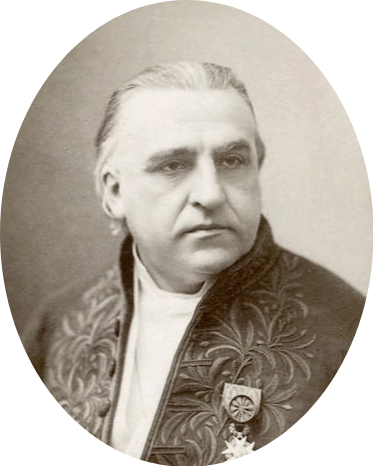
\includegraphics[width=.25\textwidth]{pic/Jean-Martin_Charcot-modified.png}
			\caption{J.-M. Charcot (1825-1893), \href{https://fr.wikipedia.org/wiki/Jean-Martin_Charcot\#/media/Fichier:Jean-Martin\_Charcot.jpg}\\
				{Wikipédia}.}
		\end{figure}
					\begin{itemize}
			\small
			\item père de la neurologie moderne
			\item hystérie, \og{}Parkinson\fg{}, \textsc{SLA}$\dots$
			\item Freud, de la Tourette, Babinski$\dots$
			%			\item Fonds Charcot sur SorbonNum\footnote{\url{https://patrimoine.sorbonne-universite.fr}}
		\end{itemize}
	\end{columns}

\end{frame}


\section[Problématique]{Problématique}
\input{objectif_double}
\begin{frame}{Double objectif}
	\begin{figure}
		\centering
		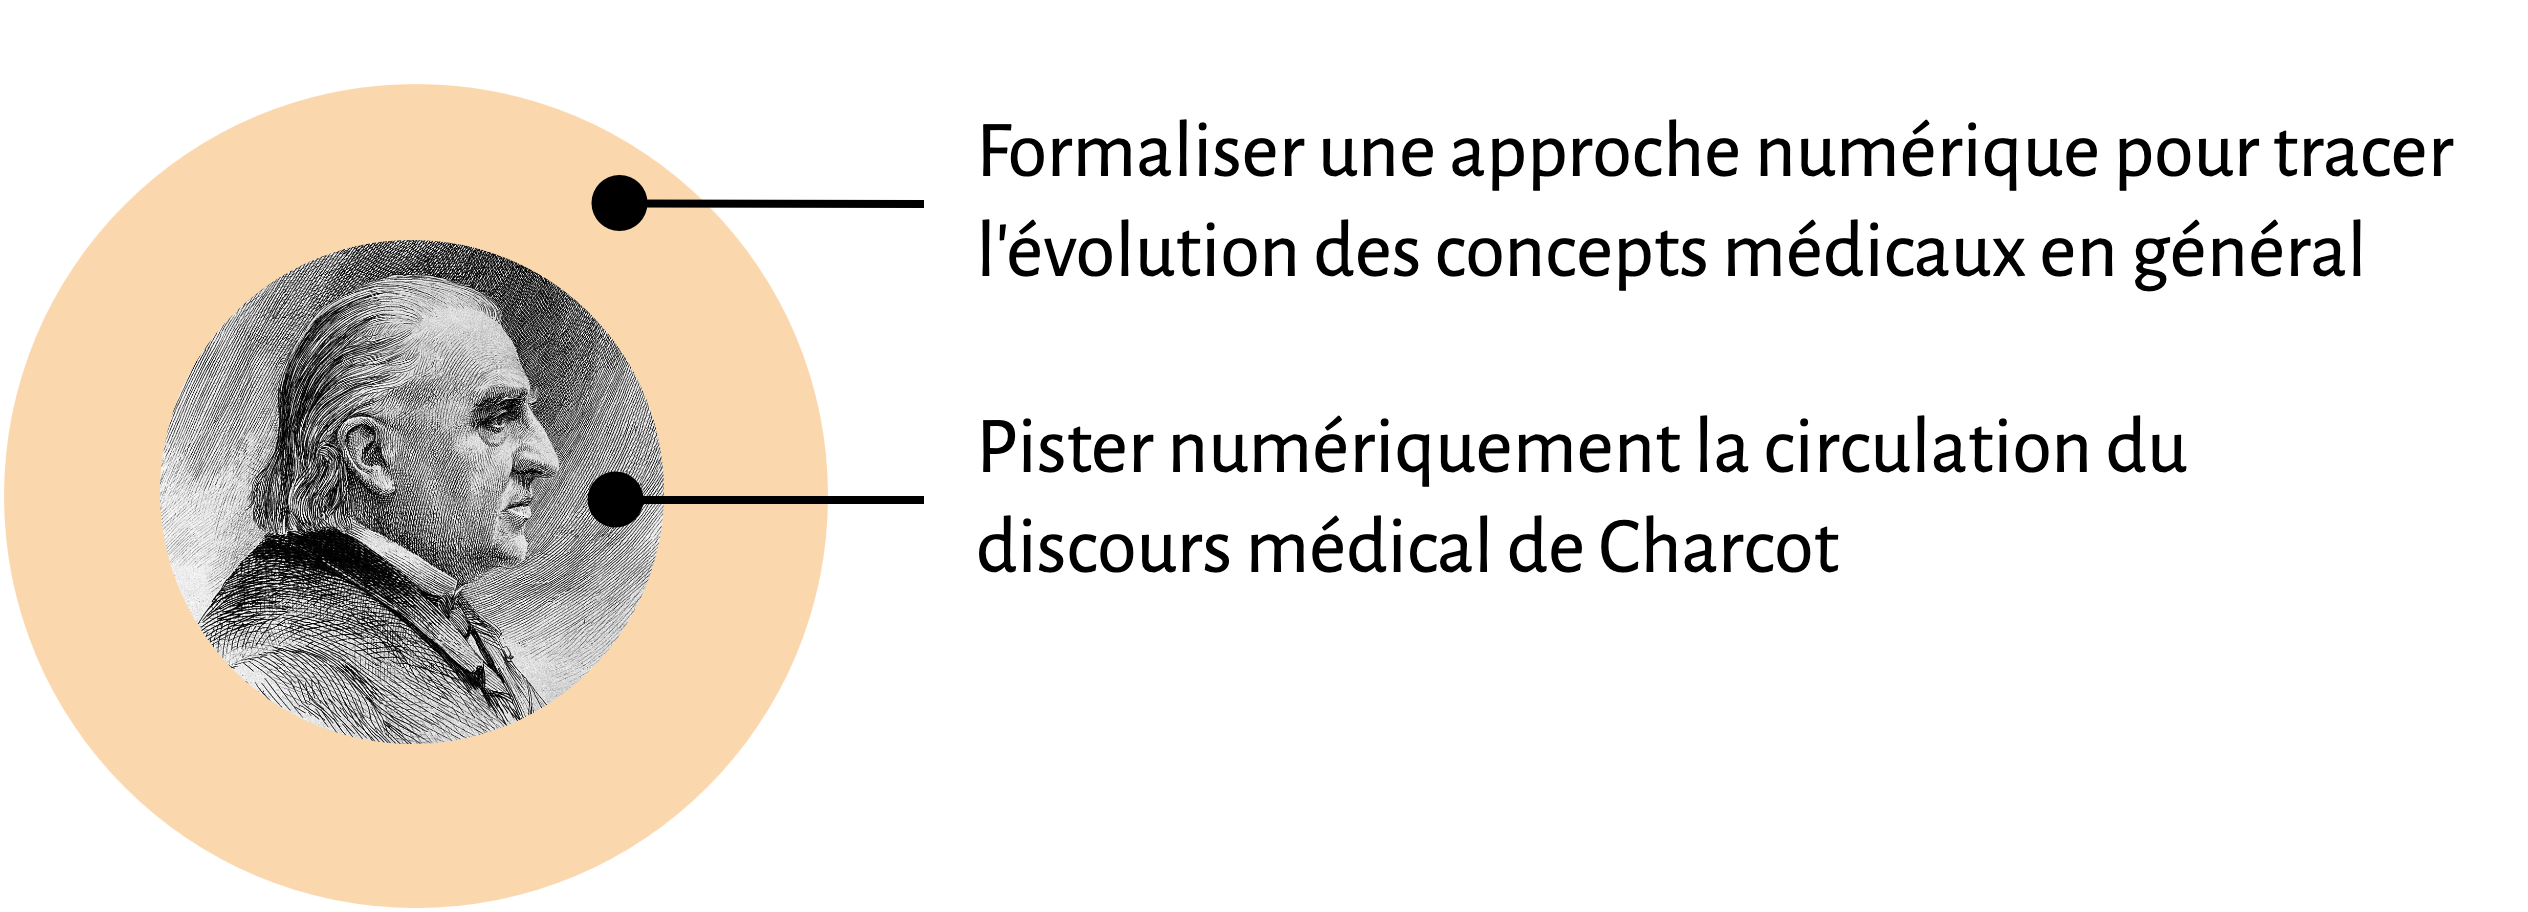
\includegraphics[width=1\textwidth]{pic/objectif_double.png}
		%\caption{}
	\end{figure}
	
	\begin{variableblock}{}{bg=white,fg=red}{bg=green,fg=pink}
		\centering
		Est-il possible de mesurer l'impact de Charcot sur son réseau scientifique\textcolor{BlueViolet}{*} en s'appuyant sur les termes scientifiques qu'il a employés ?
	\end{variableblock}
	\begin{flushright}
		{\footnotesize\textcolor{BlueViolet}{* élèves, collègues et successeurs\\
				$\rightarrow$ collaborateurs}}
	\end{flushright}
	
	
\end{frame}

\begin{frame}{Hypothèses}


	\begin{variableblock}{}{bg=white,fg=deepblue}{bg=green,fg=pink}
		\justifying
	Le texte comme point d’entrée pour étudier les tendances de la circulation des idées à l'aide des caractéristiques structurelles spécifiques \\\raggedleft\textcolor{deepred}{\citep{milia2023}}
\end{variableblock}

		\begin{variableblock}{}{bg=white,fg=deepblue}{bg=green,fg=pink}
	\justifying
	Certains \textbf{termes médicaux} dont Charcot a été l’inventeur (\textsc{SLA}) ou le transmetteur (\textit{hystérie}) ont été repris de manière significative dans les écrits de son réseau scientifique.
\end{variableblock}
\end{frame}

\begin{frame}{Recherches quantitatives des circulations des savoirs}
	%Domaine peu documenté
	Tendances de circulation linguistique dans les fronts de recherche 

	
			        \begin{figure}[!h]
		\centering
		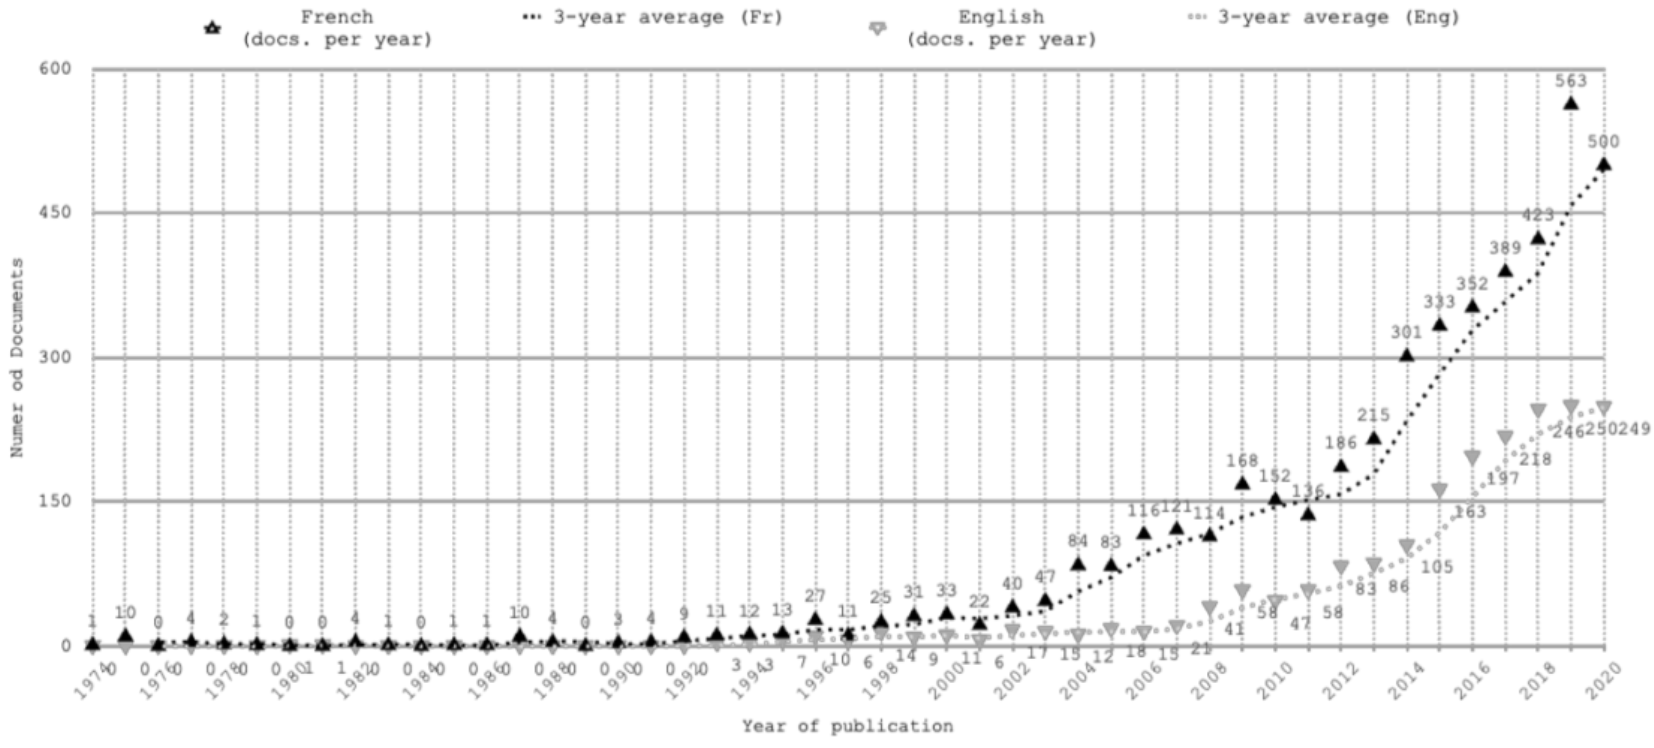
\includegraphics[width=1\textwidth]{pic/thematic_interests.png}
		\caption{Nombre de documents représentant les intérêts thématiques en anglais et en français \citep{milia2023}.}
	\end{figure}
	
\end{frame}


\begin{frame}{Recherches quantitatives des circulations des savoirs}
	%Domaine peu documenté
	Tendances de circulation linguistique dans les fronts de recherche 
	
	
	\begin{figure}[!h]
		\centering
		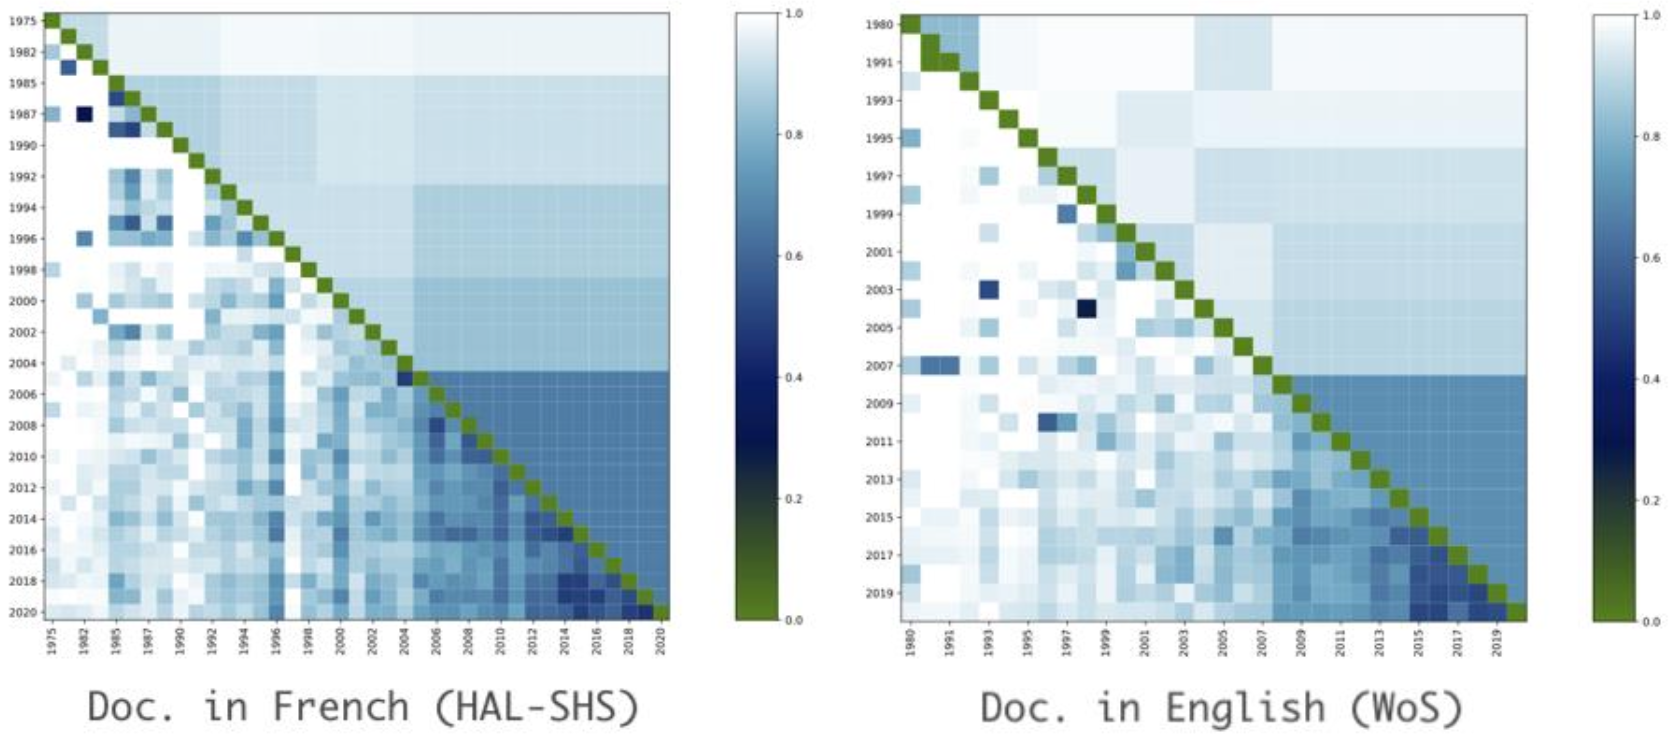
\includegraphics[width=1\textwidth]{pic/period_detection.png}
		\caption{Détection de période à l'aide d'une corrélation significative des termes au fil des années dans deux sources et langues différentes \citep{milia2023}.}
	\end{figure}
	
\end{frame}



\begin{frame}{Recherches quantitatives des circulations des savoirs}
	\begin{itemize}
	\item réception de la pensée scientifique de C. Bernard \citep{riguet2018impact}
\item détection des réemplois textuels
\citep{fedchenko2024recherche}
\item Rankingdom -- mesurer l'importance d’une entité \citep{soulet2024}
\end{itemize}
\begin{figure}[!h]
\centering
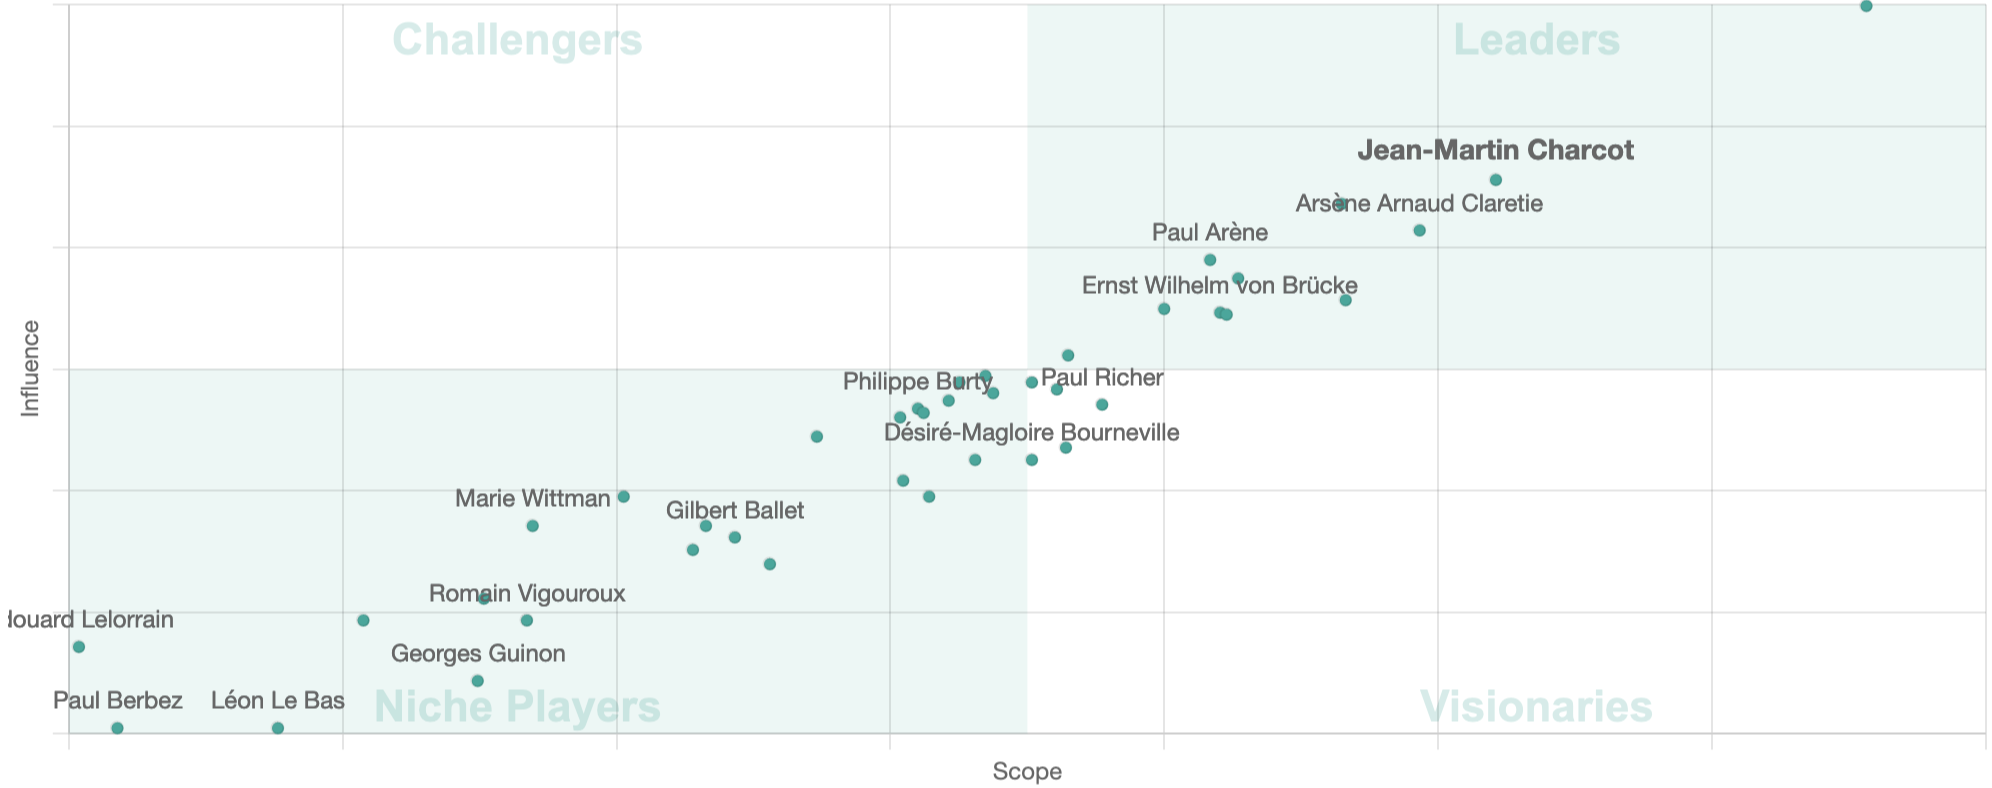
\includegraphics[width=1\textwidth]{pic/analyse_quadrant.png}
\caption{Positionnement de l'entité \texttt{Charcot} au sein de son domaine \textit{via} l'analyse de quadrant.}
\end{figure}
\end{frame}

%\begin{frame}{Impact temporel de Charcot}
%\begin{figure}[!h]
%		\centering
%		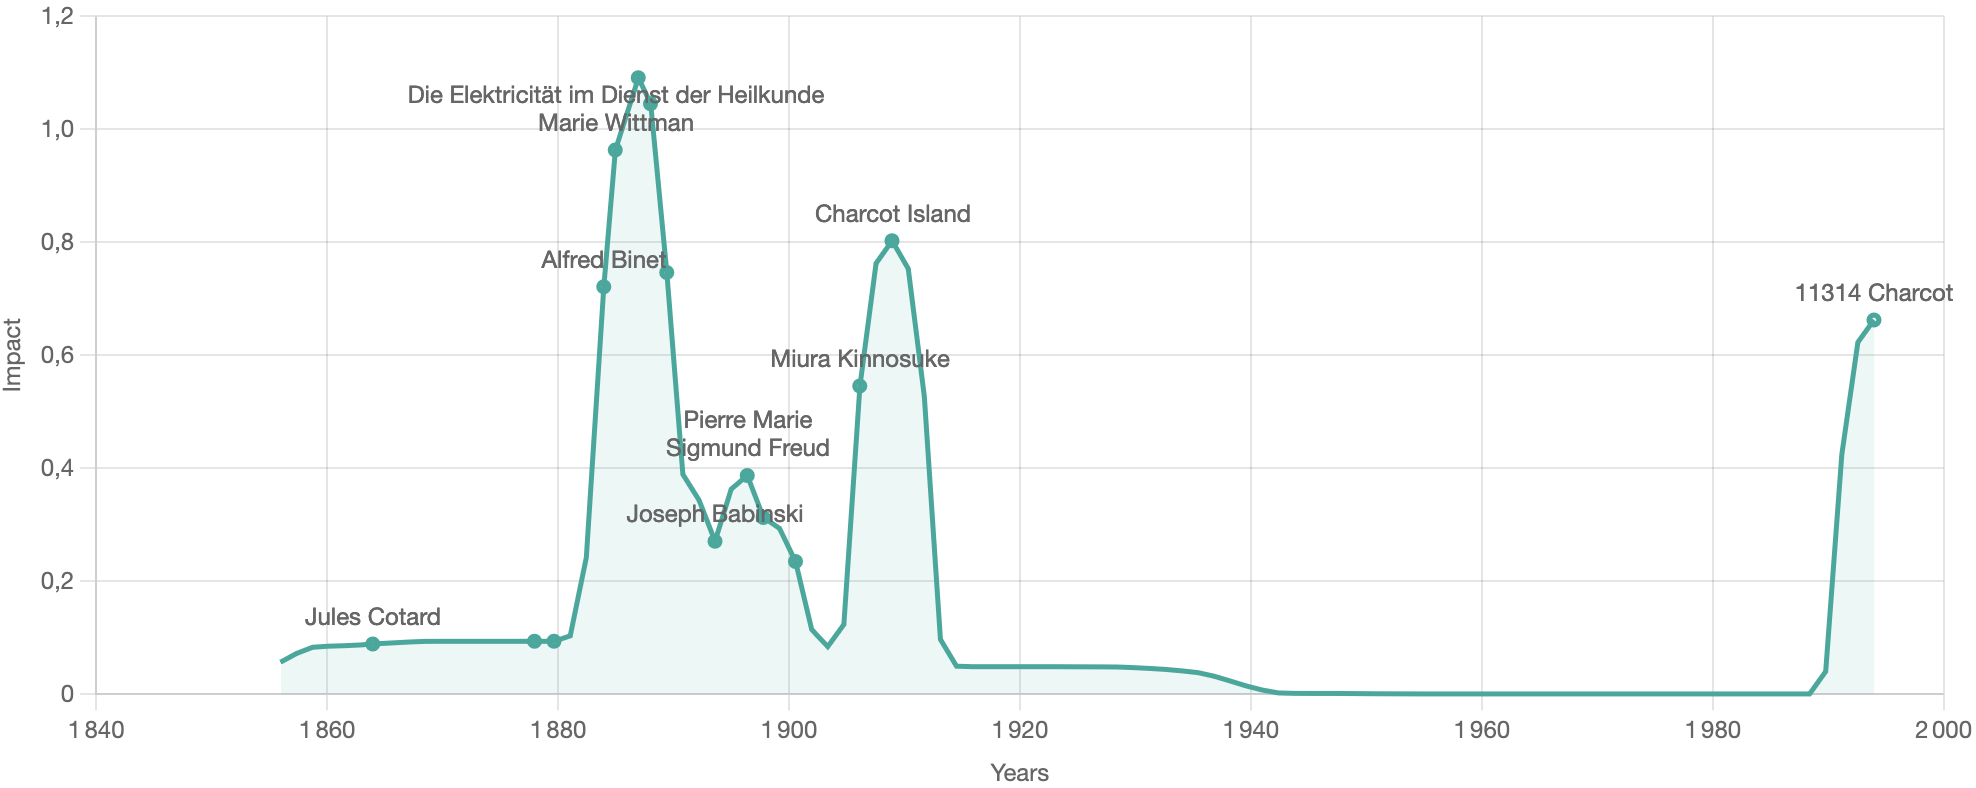
\includegraphics[width=1\textwidth]{pic/impact_temporel.png}
%		\caption{Analyse temporelle de l'impact de l'entité \texttt{Charcot} \textit{via} Rankingdom.}
%	\end{figure}
%\end{frame}





\section[Méthodologie]{Méthodologie}
\begin{frame}{Fonds Charcot\footnote{\url{https://patrimoine.sorbonne-universite.fr/collection/Fonds-Charcot}}}
	\begin{variableblock}{SorbonNum\\
			\footnotesize{Bibliothèque de Sorbonne Université (\textsc{BSU})}}{bg=white,fg=deepblue}{bg=blue,fg=pink}
		201 documents XML OCRisés (sans post-correction)
	\end{variableblock}
	%\begin{itemize}
	%    \item \textrm{Charcot} : textes rédigés par Charcot
	%    \item \textrm{Autres} : textes rédigés par les membres de son réseau scientifique
	%\end{itemize}
	\begin{table}[!ht]
		\centering
		\begin{tabular}{|c|r|r|}
			\hline 
			\rowcolor{yellow!30}
			Corpus & \multicolumn{1}{c|}{Nb de docs} & \multicolumn{1}{c|}{Nb de tokens} \\
			\hline
			\begin{tabular}[c]{@{}c@{}}\textrm{Charcot}\\ \scriptsize{textes rédigés par Charcot}\end{tabular}  & 68 & 12 190 649 (38,12\%) \\
			\hline
			\begin{tabular}[c]{@{}c@{}}\textrm{Autres}\\ \scriptsize{textes rédigés par les membres} \vspace{-0.15cm} \\ \scriptsize{de son réseau scientifique}\end{tabular}    & 133 & 19 788 830 (61,88\%) \\
			\hline\hline
			\textbf{Total} & \textbf{201} & \textbf{31 979 479} (100\%)\\
			\hline
		\end{tabular}
		\caption{Répartition du fonds Charcot selon les auteurs.
			%    \footnote{\tiny{\url{https://patrimoine.sorbonne-universite.fr/collection/Fonds-Charcot}}}
		}
		\label{tab:my_label}
	\end{table}
\end{frame}

\begin{frame}{Formalisation de l'approche}
	Extraction des concepts $\rightarrow$ problème d’extraction de la terminologie
	\begin{figure}[!h]
		\centering
		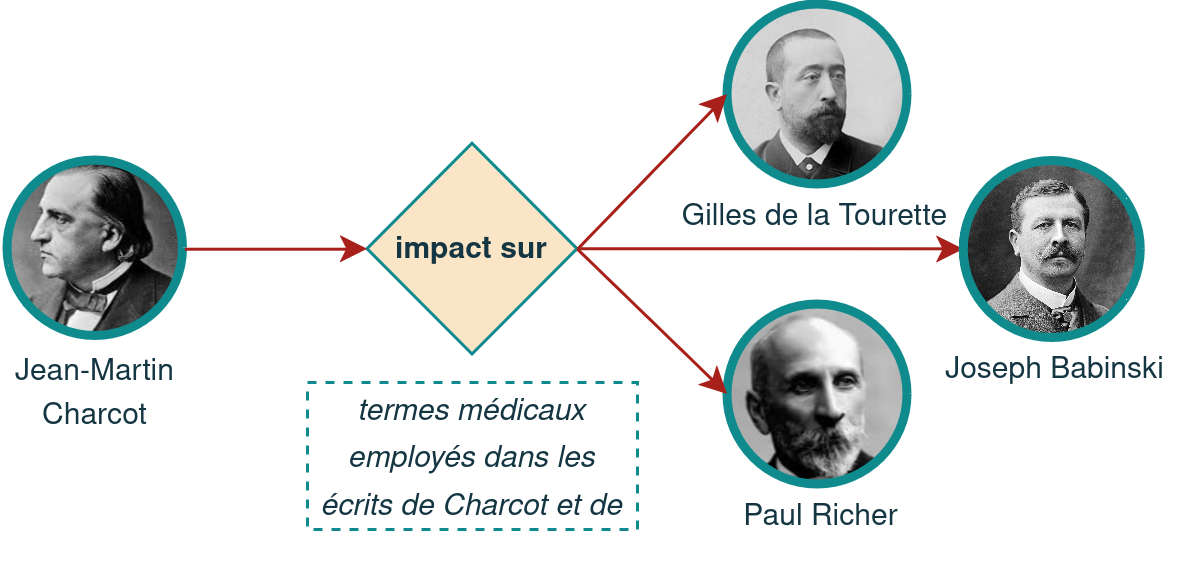
\includegraphics[width=100mm,scale=0.5]{pic/charcot_intertextualite.png}
		\caption{Opérationnalisation de l'impact de Charcot sur ses élèves.}
		\label{fig:my_label}
	\end{figure}
\end{frame}


\begin{frame}{Liste des concepts médicaux -- vérité terrain}
	Extraction semi-automatique des termes en lien avec Charcot.\\{\scriptsize\url{https://github.com/ljpetkovic/Charcot\_circulations/tree/main/concepts}}
	
	\begin{figure}[!htb]
		\centering
		\begin{minipage}{.5\textwidth}
			\centering
			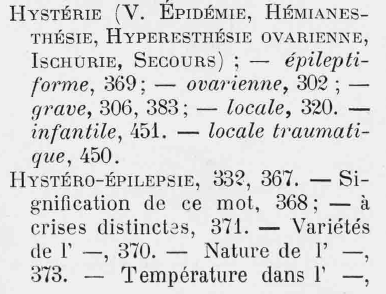
\includegraphics[width=0.6\linewidth, height=0.3\textheight]{pic/concepts-pdf}
			\caption{Index des termes \citep{charcot1892oeuvres}.}
			\label{fig:prob1_6_2}
		\end{minipage}%
		\begin{minipage}{.5\textwidth}
			\centering
			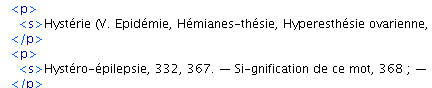
\includegraphics[width=1\linewidth, height=0.15\textheight]{pic/concepts-xml}
			\caption{Concepts médicaux, document XML.}
			\label{fig:prob1_6_1}
		\end{minipage}
	\end{figure}
 \begin{figure}[!htb]
	\centering
	\begin{minipage}{.5\textwidth}
		\centering
		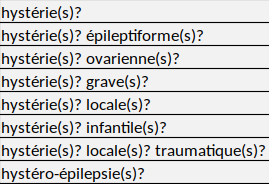
\includegraphics[width=0.6\linewidth, height=0.25\textheight]{pic/concepts-csv}
		\caption{Liste finale des concepts médicaux.}
		\label{fig:prob1_6_2}
	\end{minipage}%
	\begin{minipage}{.6\textwidth}
		\centering
		\begin{enumerate}
			\setcounter{enumi}{0}
			\item entre \texttt{<s>} et \texttt{,-(} (regex)
			\item sans termes génériques (\textit{os}, \textit{peau})
			\item prise en compte des sg. / pl. (regex)
		\end{enumerate}
	\end{minipage}
\end{figure}
\end{frame}


\input{bm25}
\input{keyphrase}

\section[Expériences]{Expériences}
\begin{frame}{Extraction de la terminologie : approche linguistique $\cdot$ \texttt{TermSuite}\footnote{\url{https://termsuite.github.io/}}\textsuperscript{,}\footnote{\url{https://github.com/ljpetkovic/Charcot\_TermSuite/tree/main}}}
	%	Corpus Charcot accessible sur la plateforme \textsc{OBVIE} \hfill {\small\citep{alrahabi2022obvie}}
	%	\begin{itemize}
		%		\item fouille avancée des corpus en \textsc{XML-TEI}
		%		\item textes similaires : mots fréquents / en commun, noms cités
		%	\end{itemize}
	%	%\danger impossible de quantifier l'importance des MWEs
	%	\begin{figure}[!h]
		%		\centering
		%		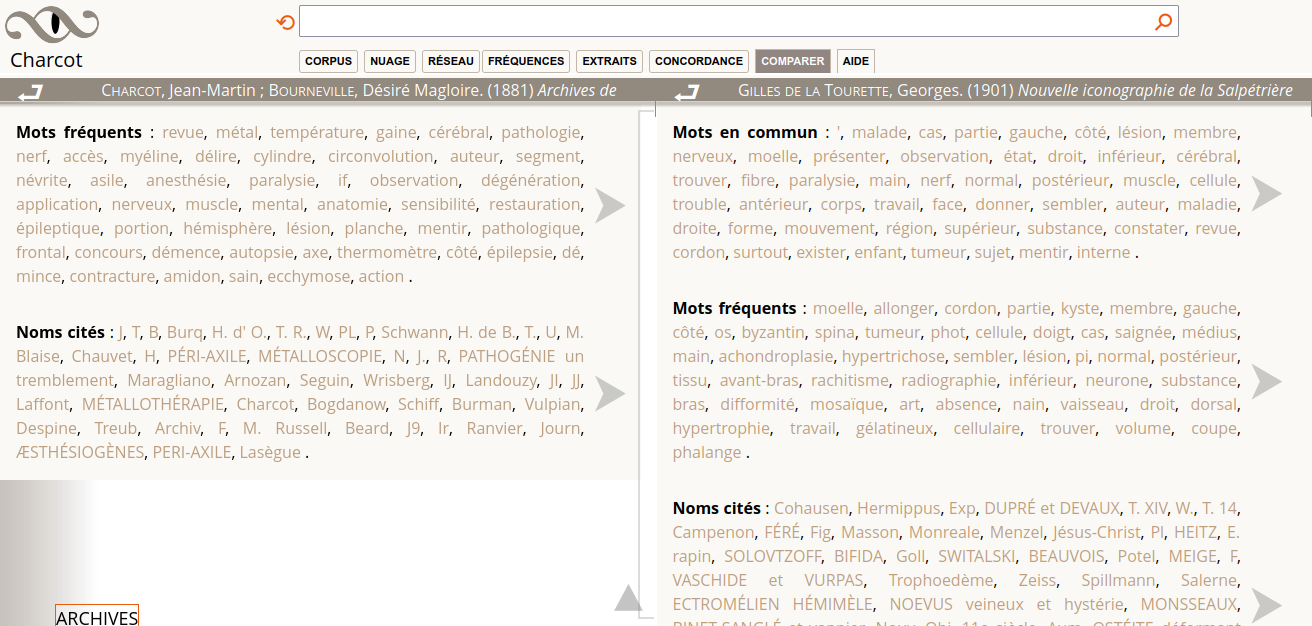
\includegraphics[width=90mm,scale=0.5]{pic/doc_sim.png}
		%		\caption{Points similaires entre un ouvrage de Charcot et celui de de la Tourette.}
		%		%    \caption{Distribution des fréquences des tokens avec la frise chronologique pour ceux constituant l'expression \textit{bulbe rachidien} (issus des corpus \og{}Charcot\fg{} et \og{}Autres\fg{}).}
		%		\label{fig:my_label}
		%	\end{figure}
	%Mesurer informatiquement l'impact de Charcot sur son \og{}réseau\fg{} \\$\rightarrow$ intertextualité uni-directionnelle
	%\begin{figure}[!h]
	%    \centering
	%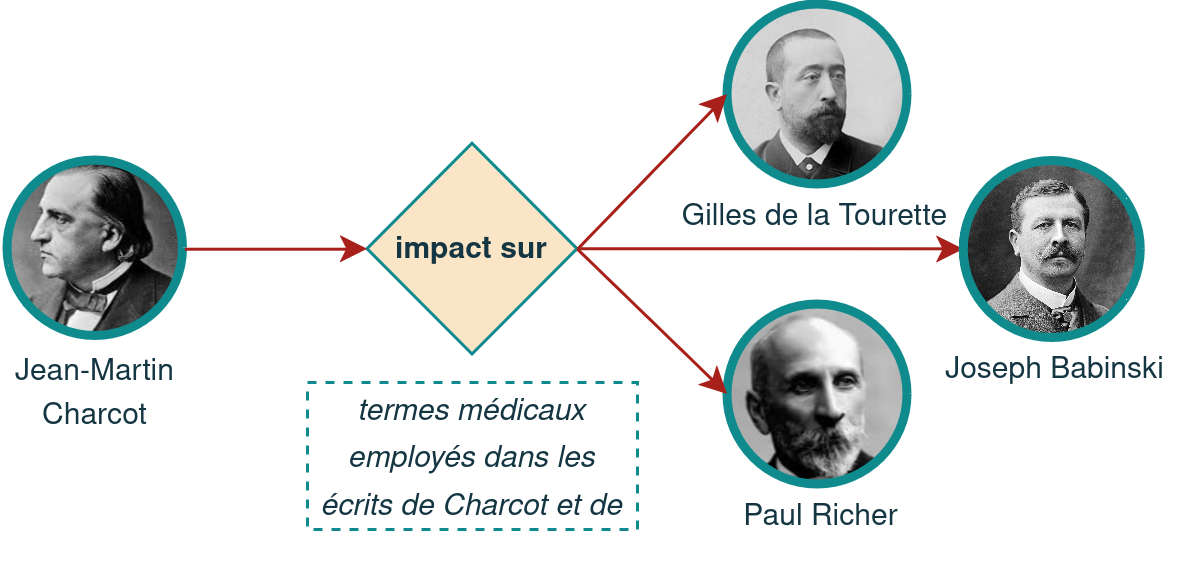
\includegraphics[width=100mm,scale=0.5]{pic/charcot_intertextualite.png}
	%    \caption{Opérationnalisation de l'impact de Charcot sur ses élèves.}
	%    \label{fig:my_label}
	%\end{figure}
	%	\begin{variableblock}{\texttt{TermSuite}\footnote{\url{https://termsuite.github.io/}}}{bg=white,fg=deepblue}{bg=white,fg=deepred}
		%		\justifying
		%%	Extraction des termes uniques et de leurs caractéristiques \begin{itemize}
			%%		\item étiquettes \textsc{POS}, fréq. brute et documentaire,  \textsc{TF-IDF}, spécificité$\dots$
			%%	\end{itemize}
		%\end{variableblock}
		Termes uniques + motifs syntaxiques (6)
		\begin{itemize}
			\item système à base de règles + mesures statistiques
			\begin{itemize}
				\item \textsc{TF-IDF}, spécificité, fréquences$\dots$
				\item 261 termes en commun
			\end{itemize} 
		\end{itemize}
		\begin{table}[h]
			\centering
			\resizebox{\textwidth}{!}{
				\begin{tabular}{|lrrr|rrl|}
					\hline\hline
					\rowcolor{gray!10}\multicolumn{4}{|c|}{Corpus Charcot}                                                                    & \multicolumn{3}{|c|}{Corpus Autres}                               \\ \hline
					\multicolumn{1}{|c|}{Motif POS}      & \multicolumn{1}{c|}{Effectif} & \multicolumn{1}{c|}{Fréq. relat. (\%)} & \multicolumn{1}{c|}{Exemple} & \multicolumn{1}{c|}{Effectif} & \multicolumn{1}{c|}{Fréq. relat. (\%)} & \multicolumn{1}{c|}{Exemple}\\ \hline
					\rowcolor{yellow!30}\multicolumn{1}{|c|}{\textsc{N}}              & \multicolumn{1}{r|}{261}               & \multicolumn{1}{r|}{52,10}                   & \multicolumn{1}{c|}{\textit{hystérie}} & \multicolumn{1}{r|}{271}               & \multicolumn{1}{r|}{54,20} & \multicolumn{1}{c|}{\textit{somnambule}}                  \\ \hline
					\multicolumn{1}{|c|}{\textsc{A}}              & \multicolumn{1}{r|}{151}               &  \multicolumn{1}{r|}{30,14}                   & \multicolumn{1}{c|}{\textit{cérébral}} & \multicolumn{1}{r|}{149}               & \multicolumn{1}{r|}{29,80}      &   \multicolumn{1}{c|}{\textit{hypnotique}}          \\ \hline
					\multicolumn{1}{|c|}{\textsc{N A}}            & \multicolumn{1}{r|}{73}                & \multicolumn{1}{r|}{14,57}                   &
					\multicolumn{1}{c|}{\textit{système nerveux}} 	& \multicolumn{1}{r|}{73}                & \multicolumn{1}{r|}{14,60}       	&
					\multicolumn{1}{c|}{\textit{lame médullaire}}            \\ \hline
					\multicolumn{1}{|c|}{\textsc{N P N}}          & \multicolumn{1}{r|}{12}                & \multicolumn{1}{r|}{2,40}                    &
					\multicolumn{1}{c|}{\textit{cas de folie}} &
					\multicolumn{1}{r|}{6}                 & \multicolumn{1}{r|}{1,20}   &
					\multicolumn{1}{c|}{\textit{scissure de sylvius}}                 \\ \hline
					\multicolumn{1}{|c|}{\textsc{N A A}}          & \multicolumn{1}{r|}{3}                 & \multicolumn{1}{r|}{0,60}                    &
					\multicolumn{1}{c|}{\textit{système nerveux central}} &
					\multicolumn{1}{r|}{0}                 & \multicolumn{1}{r|}{0,00}           &
					\multicolumn{1}{c|}{--}         \\ \hline
					\multicolumn{1}{|c|}{\textsc{R}}              & \multicolumn{1}{r|}{1}                 & \multicolumn{1}{r|}{0,20}                    &
					\multicolumn{1}{c|}{\textit{[d']emblée}} &
					\multicolumn{1}{r|}{1}                 & \multicolumn{1}{r|}{0,20}       &
					\multicolumn{1}{c|}{\textit{obliquement}}             \\ \hline\hline
					\multicolumn{1}{|c|}{\textbf{Total}} & \multicolumn{1}{r|}{\textbf{501}}      & \multicolumn{1}{r|}{100,00}                  &
					\multicolumn{1}{r|}{\cellcolor{blue!25}} &
					\multicolumn{1}{r|}{\textbf{500}}      & \multicolumn{1}{r|}{100,00} &
					\multicolumn{1}{r|}{\cellcolor{blue!25}}                 \\ \hline\hline
				\end{tabular}
			}
			\caption{Répartition des parties du discours constituant les termes médicaux dans les deux corpus.}
			\label{tab:repartition_POS}
		\end{table}
	\end{frame}
	
	
	\begin{frame}{Répartition des motifs syntaxiques}
		
		\begin{itemize}
			\item unigrammes de noms \texttt{[N]} et des adjectifs \texttt{[A]} : les plus fréquents
			\item trigrammes : les séquences les plus longues extraites
			\begin{itemize}
				\item aucune occurrence du trigramme \textit{sclérose latérale amyotrophique}\\\textcolor{deepred}{seule trace : adjectif \texttt{[A]} \textit{latérale}}
				\item \textit{idem} pour le quadrigramme \textit{état de mal hystéro-épileptique}
			\end{itemize}
			
		\end{itemize}
		
		\begin{figure}[!h]
			\centering
			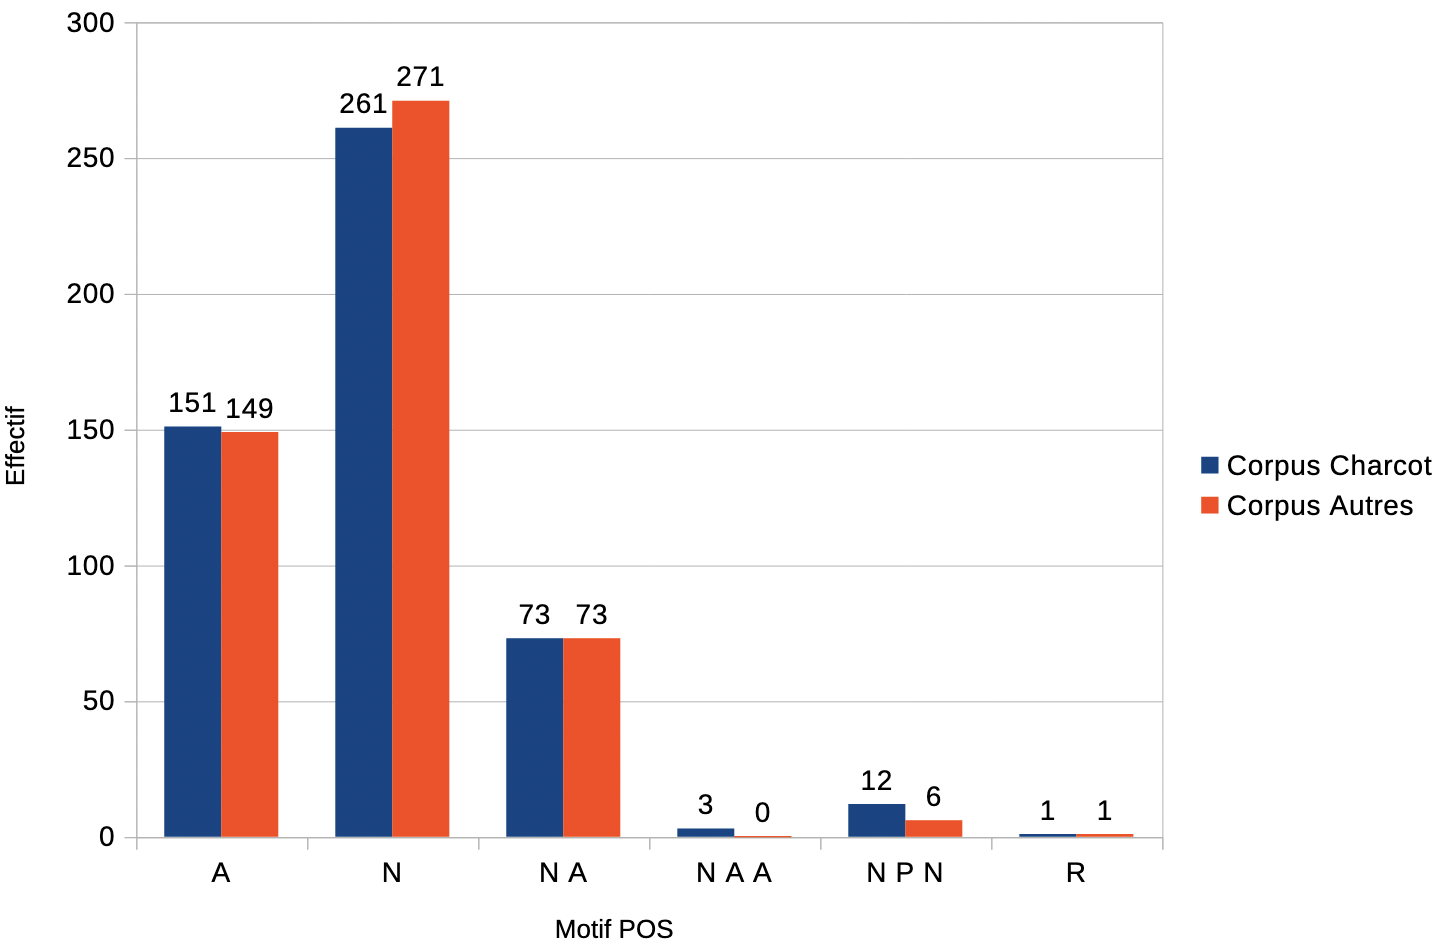
\includegraphics[width=0.65\textwidth]{pic/repartition_motifs_POS.png}
			\caption{Analyse comparative des séquences syntaxiques.}
		\end{figure}
		
	\end{frame}
	
	\begin{frame}{\textsc{TF-IDF}}
		Premiers 12 termes communs, à partir du \texttt{TF-IDF} $\approx$ \textsc{0,15}
		\begin{itemize}
			\item prévalence des unigrammes
		\end{itemize}
				\begin{figure}[!h]
			\centering
			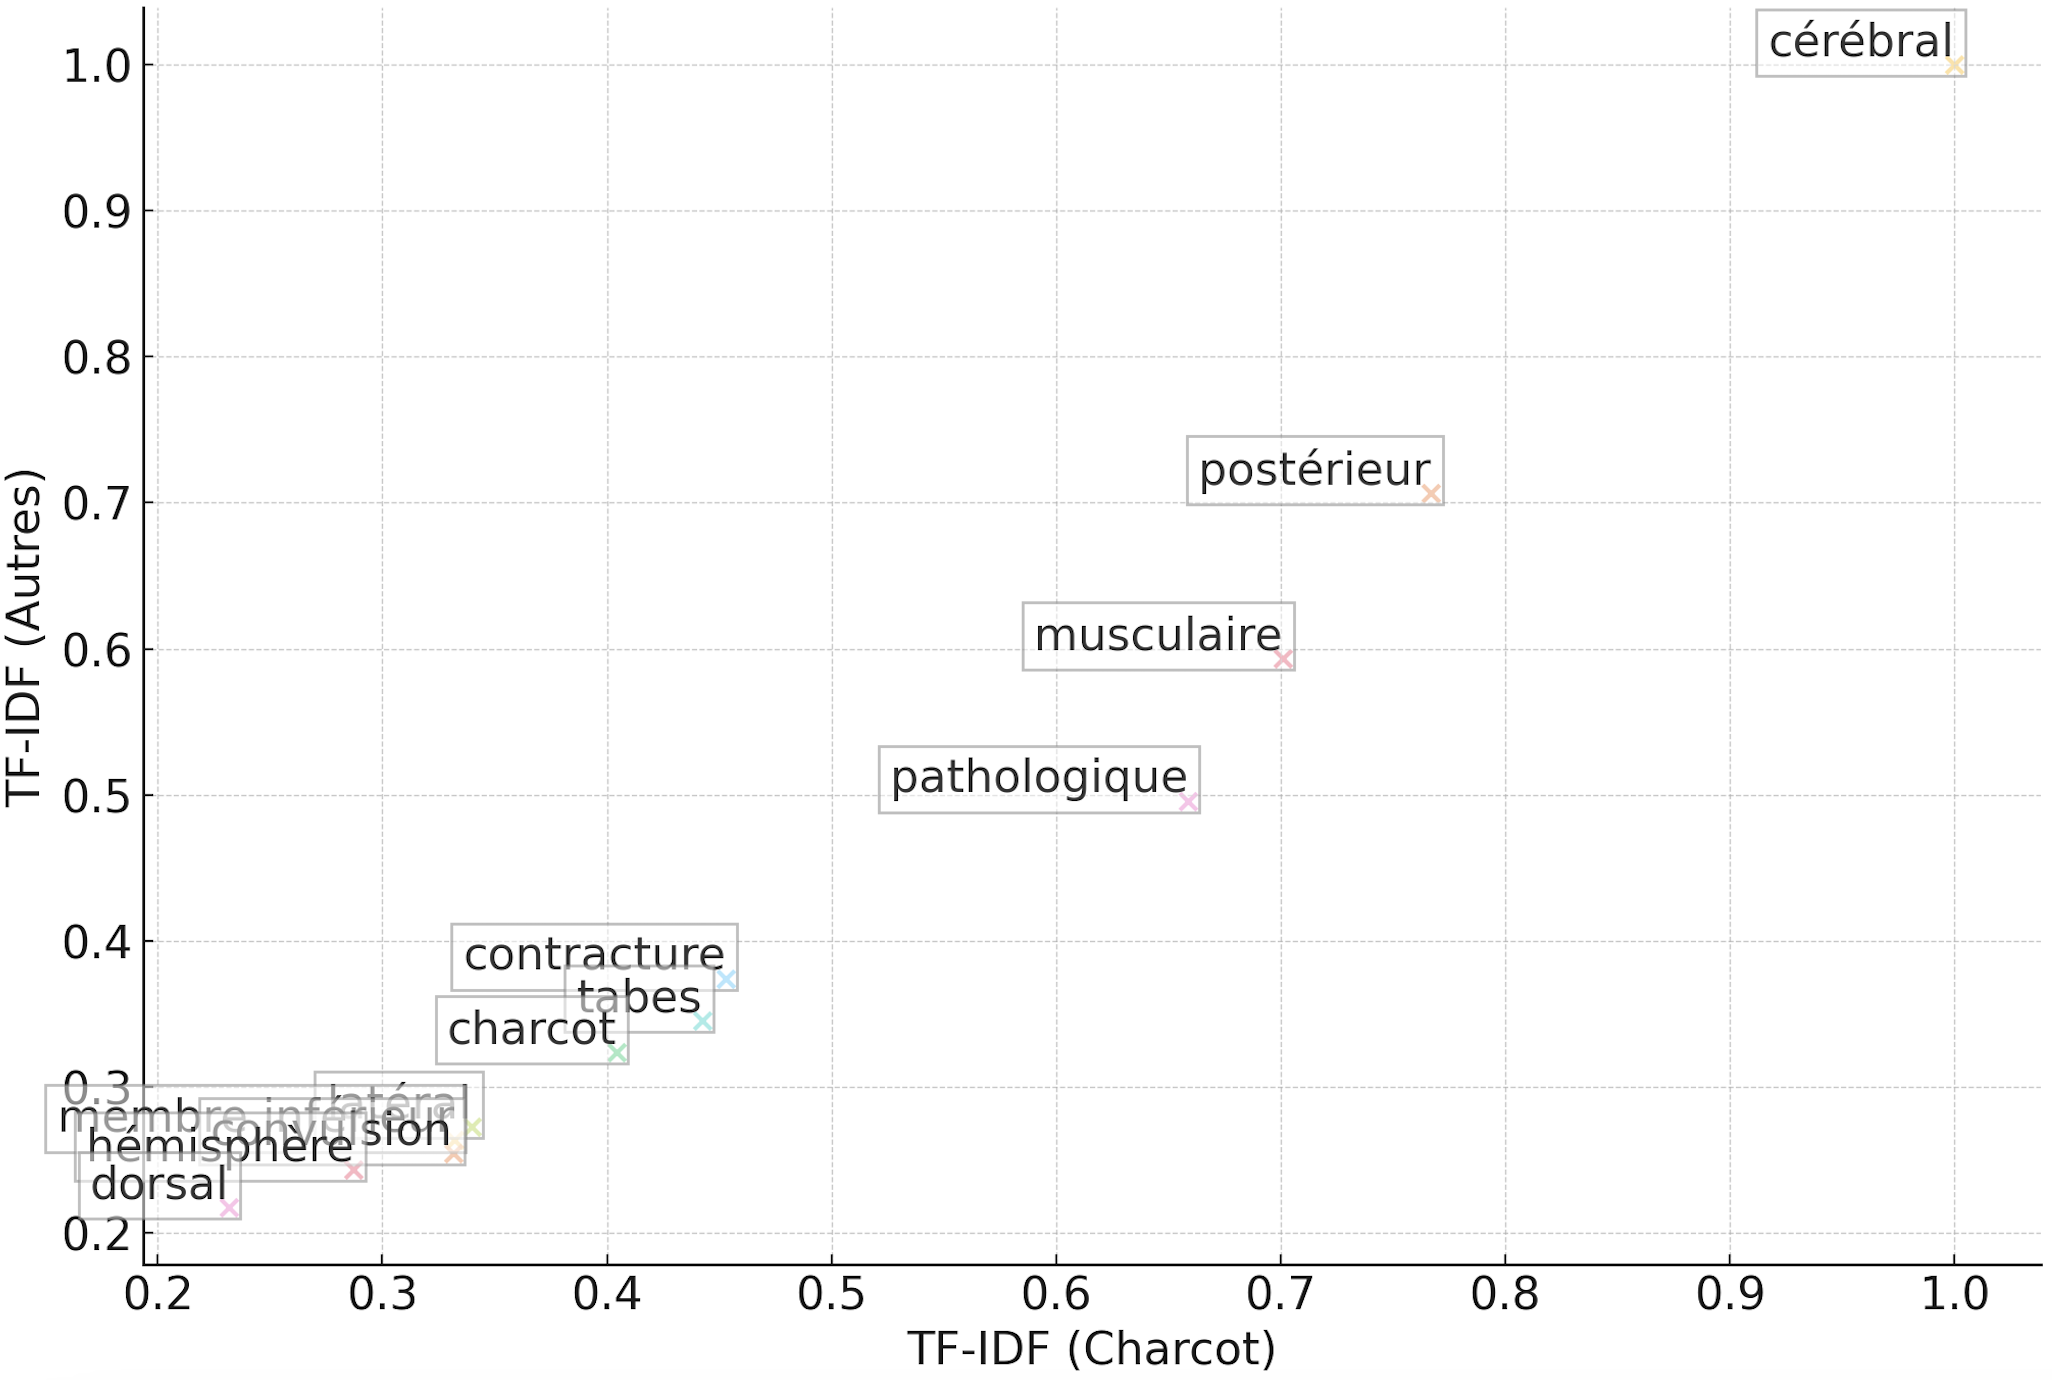
\includegraphics[width=0.7\textwidth]{pic/scatter_plot.png}
			\caption{Termes communs avec leurs valeurs \textsc{TF-IDF} respectives.}
		\end{figure}
	\end{frame}

%\begin{frame}{Corpus Charcot -- \textsc{OBVIE}}
%	
%	\begin{itemize}
%		\item Fonds Charcot sur SorbonNum\footnote{\url{https://patrimoine.sorbonne-universite.fr}}
%		\item Corpus Charcot sur \textsc{OBVIE}\footnote{\url{https://obtic.huma-num.fr/obvie/charcot/?view=corpus}}
%	\end{itemize}
%	
%	
%\end{frame}

%\begin{frame}{Extraction des phrases-clés $\cdot$ méthode supervisée}
%	\begin{figure}[!h]
%		\centering
%		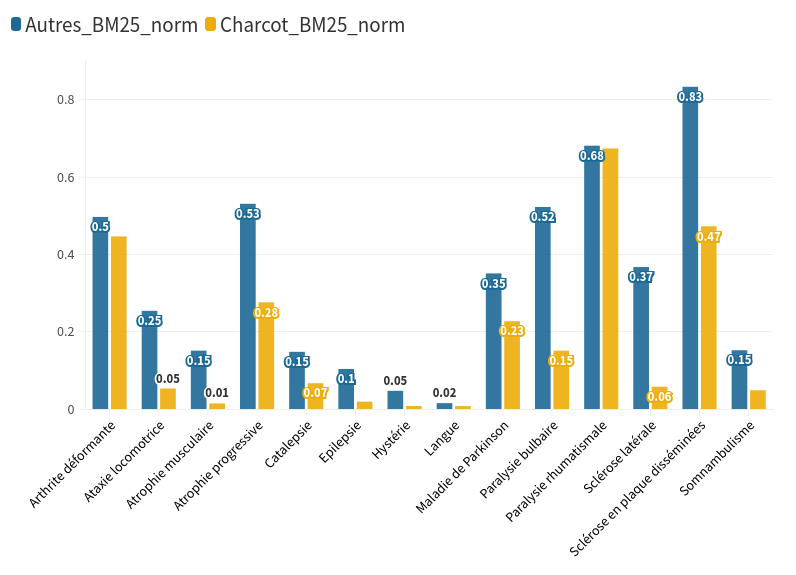
\includegraphics[width=0.6\textwidth]{pic/Charcot_Autres_250523.png}
%		\caption{Visualisation de pertinence des concepts dans les deux corpus suivant la métrique \textsc{BM25} \citep{robertson1976relevance}.}
%	\end{figure}
%	\textsc{BERT} \citep{vaswani2023} : diplopie, myélite partielle$\dots$ (Charcot)\\
%	\quad\quad\quad vicieuses, délire, miracle$\dots$ (Autres)
%\end{frame}

%\begin{frame}{Extraction des phrases-clés $\cdot$ méthode non-supervisée}
%	\begin{figure}[!h]
%		\centering
%		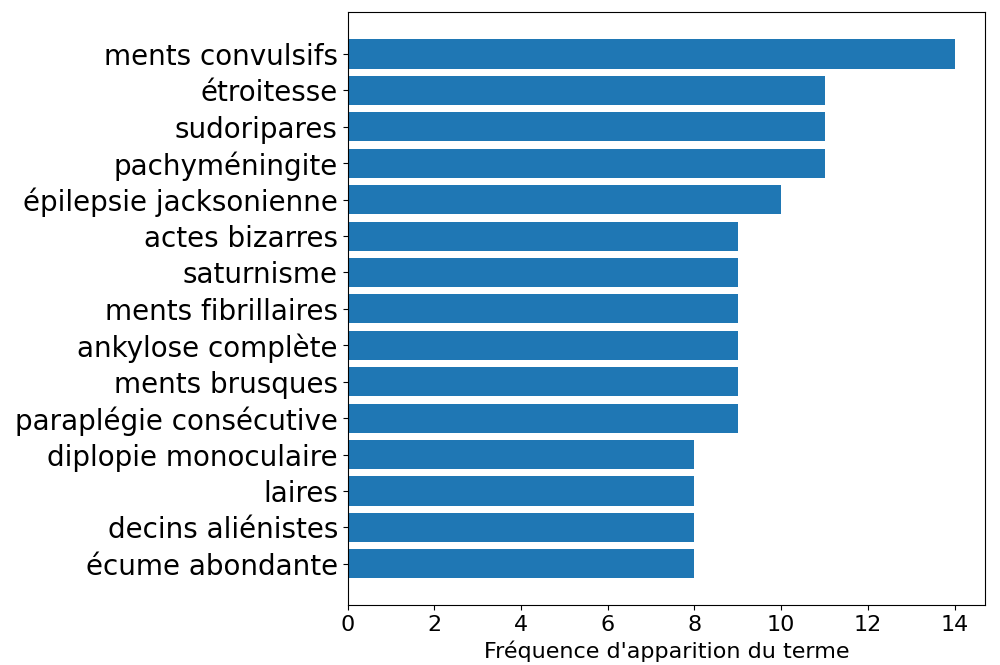
\includegraphics[width=0.8\textwidth]{pic/termes_partages.png}
%		\caption{Les 15 termes les plus fréquents partagés par Charcot et son réseau selon \texttt{keyphrase-vectorizers}\footnote{\url{https://pypi.org/project/keyphrase-vectorizers/}}.}
%	\end{figure}
%\end{frame}

\section[Conclusion]{Conclusion}
\begin{frame}{Conclusion}
	Il est possible de quantifier la pertinence des termes scientifiques partagés entre Charcot et son réseau
	\bigskip
	
	\danger Limitations de l'approche linguistique de l'extraction des termes\\$\rightarrow$ les termes plus pointus sont pénalisés
			
\bigskip
	À faire :
	\begin{itemize}
		\item rendre compte du contexte d'énonciation des termes
		\item déterminer l'approche à adopter (plongements dynamiques ? )
		\item trouver un corpus \og{}externe\fg{} : prouver la pertinence des termes détectés pour la communauté scientifique
%		\item concevoir une approche spécifique qui permette de gérer soigneusement la collection de documents, le dictionnaire de termes, ou les deux
%		\item choisir des termes spécifiques et expliquer le contexte historique, ses différentes étapes et la signification que ces termes ont pour un groupe spécifique d'experts
	\end{itemize}
\end{frame}

%\begin{frame}{Évolution du projet}
%\begin{figure}[h]
%    \centering
%    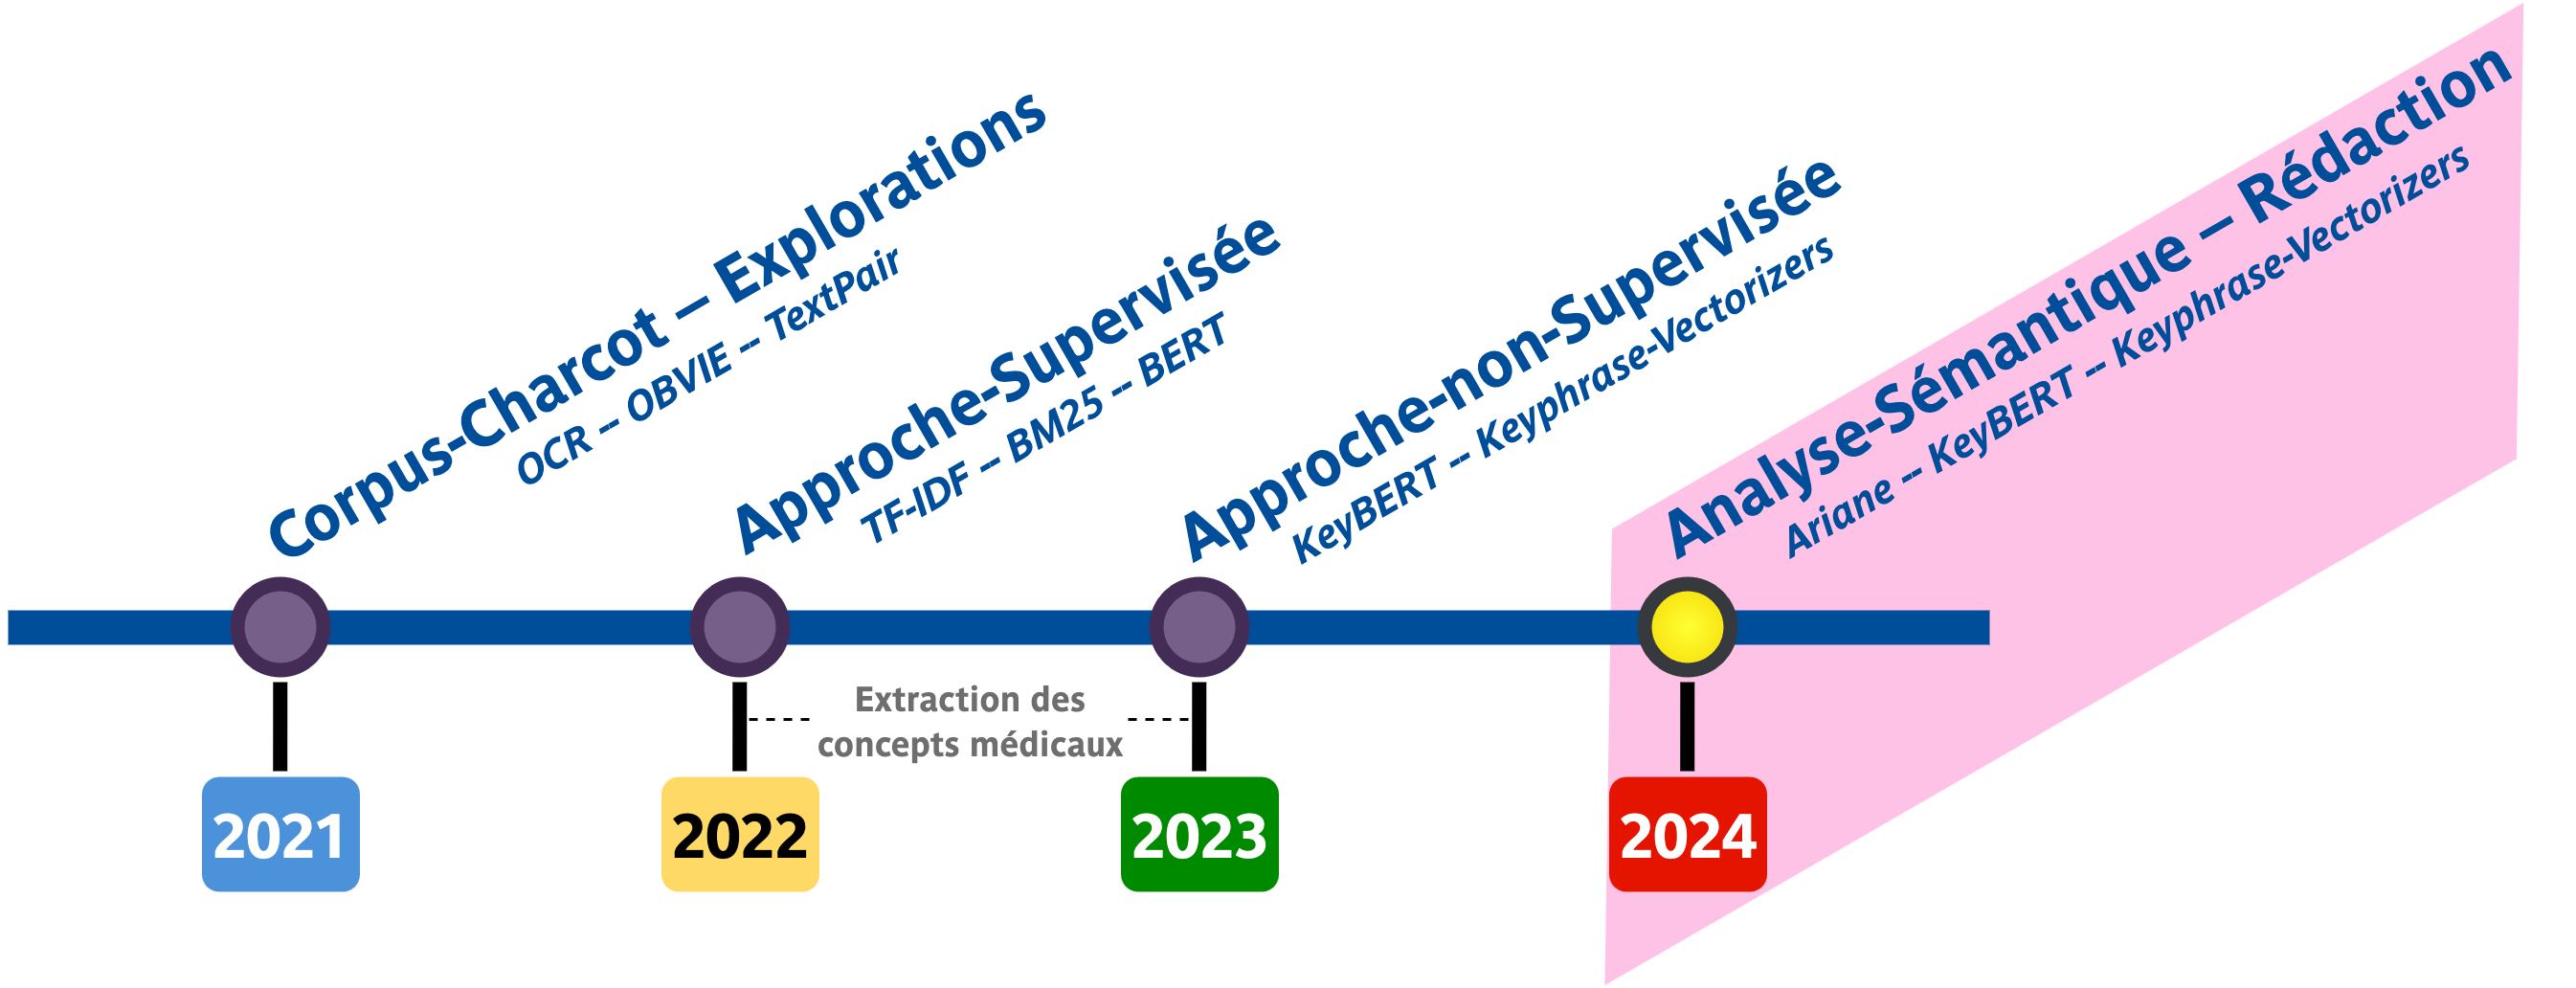
\includegraphics[width=1\textwidth]{pic/timeline_Charcot.png}
%    \label{fig:enter-label}
%    \caption{Méthodes computationnelles déjà expérimentées et à expérimenter.}
%\end{figure}
%$\rightarrow$ histoire des concepts {\footnotesize(allem. \textit{Begriffsgeschichte}) \citep{koselleck2011introduction}}
%\end{frame}


%\begin{frame}
%\frametitle{Plan}
%    \tableofcontents[sectionstyle=show,subsectionstyle=show/shaded/hide,subsubsectionstyle=show/shaded/hide]
%\end{frame}


%\section[Contexte]{Contexte de recherche}
%\input{1-1_rupture}
%\input{1-2_evolution_hysterie}
%\input{1-3_napoleon}
%\input{2-1_problematique_objectifs}
%
%\section[Objectif]{Problématique et objectif}
%\input{2-2_jonction}
%\input{2-3_question}
%
%\section[Approche supervisée]{Approche supervisée}
%\input{2_methodo}
%\input{supervise}
%\section[Approche non supervisée]{Approche non supervisée}
%\input{non_supervise}
%\section[Conclusion]{Conclusion et recherches futures}
%\input{conclusion}
%\section[État de l'art]{État de l'art}
%\input{sota}
%\section[\textit{PatternRank}]{\textit{PatternRank}}
%\input{patternrank}



% \appendix

\begin{frame}[allowframebreaks]{Références}
\printbibliography

\end{frame}

\end{document}